% FxmeNet manual. One source, two outputs:
%   make pdf    build/fxmenet-manual.pdf
%   make html   build/html/index.html (to publish on fx-mechanics.com)
% See README.md.

\documentclass[a4paper,11pt,openany,headings=small,numbers=noenddot]{scrbook}

\usepackage{fxmenet}

\usepackage[hidelinks]{hyperref}

\newcommand{\fxmenetversion}{0.1.0}

\title{\fxme\ User Manual}
\subtitle{Plugins processed on a server on your network}
\author{FX-Mechanics}
\date{Draft, \today\ (version \fxmenetversion)}

\ifdefined\HCode\else
  \usepackage[a4paper, margin=26mm]{geometry}
  \usepackage[automark,headsepline]{scrlayer-scrpage}
  \clearpairofpagestyles
  \lehead{\headmark}
  \rohead{\headmark}
  \cfoot{\pagemark}
  \addtokomafont{chapter}{\color{fxteal!60!black}}
  \addtokomafont{section}{\color{fxteal!60!black}}
  \addtokomafont{subsection}{\color{fxgrey}}
\fi

\begin{document}

\frontmatter

\begin{titlepage}
  \centering
  \vspace*{14mm}
  \fxlogo[width=0.42\textwidth]{FxmeNetLogo3.jpg}\par
  \vspace{14mm}
  {\sffamily\bfseries\Huge \fxme\ User Manual\par}
  \vspace{4mm}
  {\sffamily\Large Plugins processed on a server on your network\par}
  \vspace{16mm}
  {\large Version \fxmenetversion\par}
  \vspace{2mm}
  {\large Draft of \today\par}
  \vfill
  {\large FX-Mechanics\par}
  {\normalsize https://fx-mechanics.com\par}
\end{titlepage}

\tableofcontents

\mainmatter

\chapter{Introduction}
\label{ch:intro}

\section{What \fxme\ is}

\fxme\ lets your digital audio workstation (DAW) run its effects on another
computer. In the DAW you insert one plugin, called \ui{FxmeNet}. Behind it,
a chain of plugins runs on a \emph{server} (the program
\cmd{fxmenet-server}) on the same local network. The audio goes to the
server and comes back; the DAW sees one ordinary plugin, and compensates the
delay it reports, as it does for any plugin with latency.

The reason is simple: a session with many heavy plugins can exhaust the CPU
of the computer that runs the DAW. A second machine, even an old one, can
take that load. In our tests (chapter~\ref{ch:performance}), 24 tracks with
17 plugins each used 75\,\% of the client's processor when processed
locally, and 20 to 25\,\% through \fxme.

The server is a console program. It needs no screen, no desktop session and
no keyboard, so it can live in a cupboard or a rack, and it can run on a
different operating system than the DAW.

\section{How it works}

\fxme\ has two parts.

\begin{itemize}
  \item The \textbf{client} is the \ui{FxmeNet} plugin (VST3 and AU), loaded
    in the DAW. It has the editor you work with.
  \item The \textbf{server} is \cmd{fxmenet-server}. It loads the VST3
    plugins you ask for and processes the audio.
\end{itemize}

\begin{lstlisting}[language={}]
   Your DAW (client)                          Server
 +---------------------+                +-------------------+
 |  track 1: FxmeNet --+--- audio UDP --->  session 1: chain |
 |                     <--- audio UDP ---+  (plugin, plugin) |
 |  track 2: FxmeNet --+--- audio UDP --->  session 2: chain |
 |                     <--- audio UDP ---+                   |
 |  every instance  ---+--- control TCP -->  plugin list,    |
 |                     <-------------------  parameters, ... |
 +---------------------+                +-------------------+
\end{lstlisting}

Each instance of \ui{FxmeNet} in your project opens one \emph{session} on
the server, with its own chain of plugins. Two kinds of traffic flow:

\begin{itemize}
  \item \textbf{Audio}, in small blocks of N samples, over UDP, in both
    directions. A reply that is late is replaced by a short fade to silence
    and back (the block is \emph{concealed}); this is how a network that is
    sometimes slow stays inaudible most of the time.
  \item \textbf{Control}, over TCP: the list of plugins, adding and
    removing plugins, parameters, saving and restoring state.
\end{itemize}

The \emph{network budget} D says how many blocks of time a reply has to come
back. The latency that \fxme\ adds is about N times D samples, plus what the
DAW's own block size adds. Chapter~\ref{ch:performance} explains how to
choose them.

\section{What you see: native editors}

When you work on a plugin that sits on the server, you do not look at a
picture of a remote window. If the same plugin is installed on the client
computer, \fxme\ opens the plugin's own editor locally, and keeps it in
step with the copy on the server. Knobs respond at once, and the editor
scales with your screen. If the plugin is made for \fxme\ (see
chapter~\ref{ch:developers}), its meters and analysers show the server's
real signal. Plugins that are not installed on the client still work, with a
generic panel of sliders. These cases are the \emph{tiers} of
chapter~\ref{ch:tiers}.

\section{What \fxme\ is not}

\begin{itemize}
  \item It is not a way to play live through a very low latency. The added
    latency is a few milliseconds at best (a few tens of milliseconds for
    heavy loads). It suits mixing and production; for live monitoring,
    keep latency-critical plugins local.
  \item It is for a local network you control. The traffic is not
    encrypted and the server does not ask for a password.
    Do not expose its ports to the internet.
  \item The server hosts VST3 \emph{effects}. Instruments are not offered.
  \item It does not make plugins sound different: the server runs the same
    plugin code your DAW would run.
\end{itemize}

\section{What you need}

\begin{description}
  \item[A server.] A computer with spare CPU and a wired network
    connection. Linux is the reference platform (our tests use Ubuntu
    24.04). \todo{state which other server operating systems are supported}
  \item[A client.] A DAW on Windows, macOS or Linux that hosts VST3 (or AU on
    macOS). The tests used Reaper on Windows. \todo{list the DAWs that
    were tried}
  \item[A network.] A wired gigabit network between the two machines.
    Wi-Fi works badly for audio. A stereo track at 44.1\,kHz uses about
    3\,Mbit/s in each direction (chapter~\ref{ch:network}).
  \item[The plugins.] The plugins you want to run must be installed on the
    server. For their own editors on the client, install the same version
    there too.
\end{description}

\section{Terms used in this manual}

\begin{description}
  \item[Block size N] Samples sent to the server at a time (32 to 1024).
  \item[Network budget D] Blocks of time allowed for a reply to come back (1
    to 8).
  \item[Session] One instance of the \ui{FxmeNet} plugin, connected to the
    server, with its chain.
  \item[Chain] The plugins of a session, processed in an order you choose,
    and optionally wired by the routing (chapter~\ref{ch:routing}).
  \item[Concealed block] A block whose reply came too late, replaced by a
    short fade out and in.
\end{description}

A fuller list is in the glossary (chapter~\ref{ch:glossary}).

\chapter{Quick start}
\label{ch:quickstart}

This chapter takes you from nothing to audio going through a plugin on the
server, in about ten minutes.

\section{Get the software}

\fxme\ is built from source for now. You need a C++17 compiler, CMake 3.22 or
newer, and the JUCE framework. From the \fxme\ folder:

\begin{lstlisting}
cmake -S . -B build
cmake --build build --target FxmeNetServer -j2
cmake --build build --target FxmeNetPlugin_VST3 -j2
cmake --build build --target FxmeNetTop -j2
\end{lstlisting}

This gives three programs: the server (\cmd{fxmenet-server}), the plugin
(\file{FxmeNet.vst3}) and the monitoring tool (\cmd{fxmenet-top},
chapter~\ref{ch:top}). \todo{where the build leaves the files; how JUCE and
FxmeTools are found (sibling clones or pinned versions)}

\section{Install the plugins on the server}

The server offers the VST3 effects it finds in its plugin folders: the
standard VST3 folders of the machine (on Linux, typically
\file{~/.vst3}, \file{/usr/lib/vst3} and
\file{/usr/local/lib/vst3}), plus any you add (section~\ref{sec:folders}).
Install the plugins you want to use there, the way you would on any computer.

\section{Start the server}

On the server machine, in a terminal:

\begin{lstlisting}
fxmenet-server
\end{lstlisting}

The first time, the server examines every plugin it finds (this can take a
minute for a large collection) and then logs the list, ending with lines like:

\begin{lstlisting}[language={}]
2026-11-10 14:02:11  48 plugins (48 examined, 0 from the cache, 0 failed)
2026-11-10 14:02:11  listening: control TCP 54322, audio UDP 54321, discovery UDP 54320
\end{lstlisting}

Later starts are quick, because only new or changed plugins are examined
again. Leave the server running. Stop it with \key{Ctrl}+\key{C}.

\begin{note}
Your computers' firewall must let the three ports through on the local
network (chapter~\ref{ch:network}). Under Ubuntu's \cmd{ufw}, for example,
allow 54320 to 54322.
\end{note}

\section{Install the plugin on the client}

Copy \file{FxmeNet.vst3} to your VST3 folder on the computer that runs the
DAW (on Windows, \file{C:\Program Files\Common Files\VST3}), then let your DAW rescan its plugins.
On macOS the plugin is also built as an Audio Unit. The AU is not notarized, so macOS may refuse to load it at first; the \file{README} on the project's GitHub page explains what to do. The AU has not been tested yet, and feedback is welcome.

\section{Your first chain}

\begin{enumerate}
  \item In the DAW, add \ui{FxmeNet} to a track, as an effect.
  \item Click \ui{Find}. The server answers on the local network; choose it
    in the list. (If it does not appear, type its address in the field, for
    example \cmd{192.168.1.20}.)
  \item Click \ui{Connect}. The status line next to the button says when
    the session is ready.
  \item The list \ui{SERVER PLUGINS} shows what the server offers. Type a few
    letters of a plugin's name in the \ui{Filter} field, and press
    \key{Return} (or double-click a plugin) to add it to the chain.
  \item Play. The audio goes through the server. The plugin's controls
    appear in the right-hand panel; its parameters are also listed in the
    DAW as automation parameters.
\end{enumerate}

The line at the bottom of the editor shows the latency that \fxme\ reports to
the DAW and the count of concealed blocks. On a healthy network the count
stays at zero, or nearly.

\begin{tip}
To see what the server is doing, open \cmd{fxmenet-top} in a terminal on the
server (chapter~\ref{ch:top}). It shows each session, the server's load and
the traffic.
\end{tip}

\section{Where to go next}

\begin{itemize}
  \item Choosing the block size and budget, and making the server
    reliable: chapter~\ref{ch:performance}.
  \item Parallel chains, sidechains and multichannel plugins:
    chapter~\ref{ch:routing}.
  \item Something does not work: chapter~\ref{ch:troubleshooting}.
\end{itemize}

\chapter{The server}
\label{ch:server}

\cmd{fxmenet-server} is a console program with no window. It hosts plugins
for any number of clients at once, as far as the CPU allows.

\section{Command line}

\begin{lstlisting}
fxmenet-server [--name NAME] [--control-port N] [--udp-port N]
               [--discovery-port N] [--no-discovery]
               [--plugin-path DIR]... [--no-default-paths] [--rescan]
               [--remote-admin]
\end{lstlisting}

\begin{longtable}{@{}p{0.34\textwidth}p{0.6\textwidth}@{}}
\toprule
\textbf{Option} & \textbf{Meaning}\\
\midrule
\endhead
\cmd{--name NAME} & The name shown to clients. Default: the computer's name.\\
\cmd{--control-port N} & TCP port for control. Default 54322.\\
\cmd{--udp-port N} & UDP port for audio. Default 54321.\\
\cmd{--discovery-port N} & UDP port answering \ui{Find}. Default 54320.\\
\cmd{--no-discovery} & Do not answer \ui{Find}. Clients must then type the address.\\
\cmd{--plugin-path DIR} & Also search this folder, for this run only. May be repeated.\\
\cmd{--no-default-paths} & Do not search the standard VST3 folders, for this run only.\\
\cmd{--rescan} & Ignore the plugin cache and examine every plugin again.\\
\cmd{--remote-admin} & Let \cmd{fxmenet-top} change the plugin folders from other machines (section~\ref{sec:admin}).\\
\bottomrule
\end{longtable}

The server logs to its standard output, with a time stamp on each line, so a
service manager (such as systemd's journal) collects it.

\section{Which plugins the server offers}
\label{sec:catalog}

The server offers VST3 \emph{effects}. Instruments are skipped. A plugin
bundle that holds several plugins (a suite) offers each of them.

Each plugin file is examined in a separate process. A plugin that crashes or
hangs while it is loaded is logged, skipped, and does not take the server
down. It stays skipped until the file changes. The results are kept in a
cache file (\file{fxmenet-server-plugins.xml}, in the \file{FX-Mechanics}
folder of the user's configuration directory), keyed by the file's path, size
and date, so only new or changed plugins are examined at the next start. This
examination also notes whether the plugin is made for \fxme\
(chapter~\ref{ch:developers}).

If the same plugin is installed in two folders, the first one found is used.

\section{Plugin folders}
\label{sec:folders}

The server searches three kinds of folders:

\begin{description}
  \item[Default folders.] The standard VST3 folders of the operating system.
    They can be turned off.
  \item[Saved folders.] Folders you add with \cmd{fxmenet-top}
    (chapter~\ref{ch:top}). The server remembers them from one run to the
    next, in \file{fxmenet-server-settings.json} beside the cache file.
  \item[This run's folders.] Those given with \cmd{--plugin-path}. They are
    not remembered.
\end{description}

Folders are searched with their subfolders. After a change of folders, or
when you install a plugin while the server runs, ask for a rescan in
\cmd{fxmenet-top}. The scan runs in the background; the sessions in progress
keep playing. A client sees the new list the next time it connects.

\section{Ports and discovery}

The server listens on three ports (chapter~\ref{ch:network}). \ui{Find}
in the plugin broadcasts a question on the discovery port, and every server
answers with its name, system and number of sessions. Broadcasts normally
stay inside one network segment: across routers or VPNs, type the address.
Only one server can run on a machine with discovery on; a second one says so
in its log and runs without it.

\section{Sessions}

A session starts when a client connects and ends when it says goodbye. If a
client's connection drops (a network hiccup, a DAW that crashes), the server
keeps the session for 10 seconds, so that the client can resume it without
losing its chain.

Each session has its own audio thread. The server asks the operating system
to run it with real-time priority; if the system refuses, the server logs a
warning and runs it as an ordinary thread, which is less reliable under load
(section~\ref{sec:linuxtuning}).

\section{Reading the log}
\label{sec:log}

At startup the log lists the plugins found. Every 10 seconds, for each
session that is working, it prints one line of figures (the numbers
below are an example):

\begin{lstlisting}[language={}]
session 3: 8123 blocks, lost 0, stale 0, from cache 0, queue full 0,
send errors 0, resets 1 | process 412 us, max 10 s 1180 us, max 2310 us |
turnaround max 10 s 1650 us, over 1 block 0, over 2 blocks 0 |
chain latency 256, telemetry frames 240, parameter changes 12
\end{lstlisting}

Counts are since the session started; the values marked \emph{10 s} cover the
last interval.

\begin{longtable}{@{}p{0.27\textwidth}p{0.67\textwidth}@{}}
\toprule
\textbf{Figure} & \textbf{Meaning}\\
\midrule
\endhead
blocks & Blocks processed.\\
lost & Blocks that never arrived in time: the server skipped them (the client conceals them).\\
stale & Late blocks too old to answer, dropped.\\
from cache & Duplicate requests answered from the server's cache of recent replies.\\
queue full & Requests refused because the session could not keep up.\\
send errors & Replies the system refused to send, typically because the send buffer was full (section~\ref{sec:linuxtuning}).\\
resets & Times the client asked to restart the chain's audio (transport start, stop or jump).\\
process & Time spent processing the last block, then the worst in the last 10 seconds, then the worst since the start.\\
turnaround & Time from a request's arrival to its reply leaving, worst of the last 10 seconds.\\
over 1 block, over 2 blocks & Replies that left more than one (two) block durations after the request arrived: the server fell behind.\\
chain latency & Latency of the chain, in samples.\\
\bottomrule
\end{longtable}

A \emph{process} time that gets close to the block's duration (2.9\,ms for 128
samples at 44.1\,kHz) means the server is running out of CPU for that
session.

\section{Running the server as a service}

Below is an example of a \cmd{systemd} unit for Linux. Running the server as a service is a possibility that has not been tested yet, so treat the example as a starting point. Feedback is welcome, and so are equivalents for other systems (launchd on macOS, a Windows service).

\begin{lstlisting}[language={}]
[Unit]
Description=FxmeNet server
After=network-online.target
Wants=network-online.target

[Service]
ExecStart=/usr/local/bin/fxmenet-server
User=fxmenet
Group=audio
Restart=on-failure
LimitRTPRIO=95
LimitMEMLOCK=infinity

[Install]
WantedBy=multi-user.target
\end{lstlisting}

\section{Letting a remote \cmd{fxmenet-top} change the folders}
\label{sec:admin}

\cmd{fxmenet-top} can watch a server from any machine of the network. It may
change the plugin folders only when it connects from the server's own
machine, unless you start the server with \cmd{--remote-admin}. Because the
network is not authenticated, use this option only on a network you
trust.

\chapter{Monitoring with \cmd{fxmenet-top}}
\label{ch:top}

\cmd{fxmenet-top} is a terminal program that shows what a server is doing, in
the manner of \cmd{top}. It runs on Linux, macOS and Windows 10 or later,
in any terminal that understands ANSI escape sequences. It connects to the
server's control port as a monitor: it opens no session and never touches
the audio, so it can be started and stopped at will.

\section{Starting it}

\begin{lstlisting}
fxmenet-top                      # the server on this machine
fxmenet-top 192.168.1.20         # a server elsewhere (port 54322)
fxmenet-top studio.local:54322   # with a port
fxmenet-top --once               # print one frame without colours, and exit
fxmenet-top --find               # list the servers on the local network
\end{lstlisting}

If the server stops, \cmd{fxmenet-top} says so and reconnects when it
returns. To disable colours, set the environment variable \cmd{NO_COLOR}.

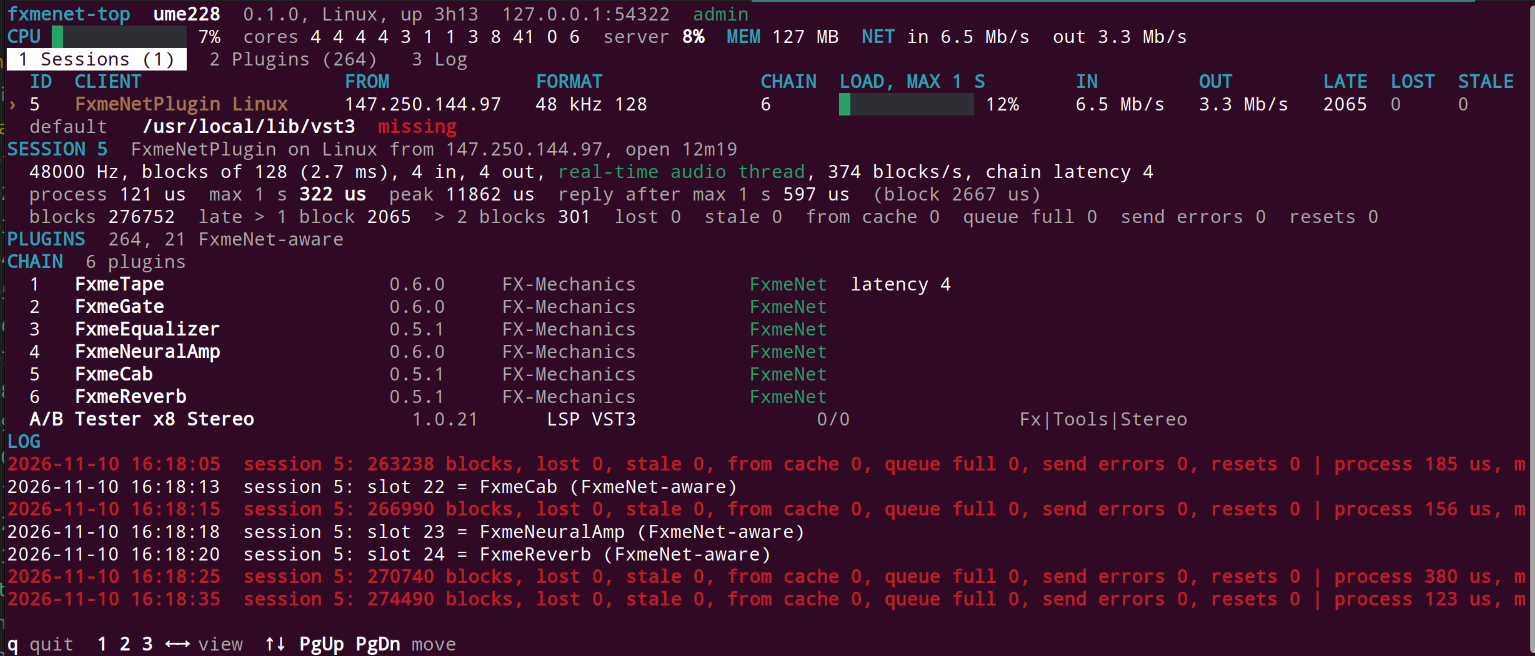
\includegraphics[width=\textwidth]{../img/fxme-net-top.png}


\section{The header}

Two lines are always visible. The first gives the server's name, version,
system and uptime, the address, and whether you may change the plugin folders
(\emph{admin}) or only watch (\emph{read only}). The second gives:

\begin{itemize}
  \item \textbf{CPU}: the machine's total use, each core, and the server
    process's use (100\,\% is one core fully used, as in \cmd{top}). Windows
    does not give the per-core figures.
  \item \textbf{MEM}: the server process's memory.
  \item \textbf{NET}: the audio traffic received and sent.
\end{itemize}

Below them, three views are selected with \key{1}, \key{2} and \key{3} (or the
left and right arrows).

\section{Sessions}

\key{1}. One line per client session: its name and system, its address, the
format (sample rate and block size), the number of plugins, a bar for the
load, the traffic, and the counts of late, lost and stale blocks. The load
bar compares the worst processing time of the last second with the block's
duration: green is comfortable, yellow is getting tight, red means the
server is close to missing deadlines. A count that has just moved turns red
for ten seconds.

Choose a session with the up and down arrows. Under the list, the details
show the format, whether the audio thread has real-time priority, the
processing times, all the counters, and the session's chain with each
plugin's version, vendor and latency. The latest log lines fill the rest of
the screen.

\section{Plugins and folders}

\key{2}. The folders the server searches (default, saved, and given on the
command line), with missing ones marked; the progress of the scan in
progress; and the plugins found, sorted by name. Press \key{/} to filter
them, as in the plugin's own list; \key{Esc} clears the filter.

When you are allowed to (\emph{admin}), these keys change the folders:

\begin{longtable}{@{}p{0.2\textwidth}p{0.74\textwidth}@{}}
\toprule
\textbf{Key} & \textbf{Action}\\
\midrule
\endhead
\key{a} & Add a folder (type an absolute path on the server, then \key{Return}).\\
\key{d} & Remove the selected saved folder.\\
\key{x} & Turn the default VST3 folders on or off.\\
\key{r} & Rescan: new or changed plugins only.\\
\key{R} & Full rescan, ignoring the cache.\\
\key{Tab} & Move between the list of folders and the list of plugins.\\
\bottomrule
\end{longtable}

The scan runs in the background and its progress appears at once. Folders
you add are kept by the server for its next runs.

\section{Log}

\key{3}. The server's log, with the latest lines at the bottom. Scroll with
the arrows, \key{PgUp} and \key{PgDn}; \key{End} follows the newest line again.
Lines that contain \emph{error}, \emph{warning} or \emph{skipped} are red.
\key{/} filters the lines.

\section{Keys}

\begin{longtable}{@{}p{0.28\textwidth}p{0.66\textwidth}@{}}
\toprule
\textbf{Key} & \textbf{Action}\\
\midrule
\endhead
\key{1} \key{2} \key{3} or arrows & Choose the view.\\
\key{Up} \key{Down} \key{PgUp} \key{PgDn} & Move in the list.\\
\key{Home} \key{End} & First or last entry (in the log, the newest).\\
\key{/} & Filter the plugins or the log.\\
\key{Esc} & Clear the filter, or cancel typing.\\
\key{q} & Quit.\\
\bottomrule
\end{longtable}

\chapter{The \ui{FxmeNet} plugin}
\label{ch:plugin}

This chapter walks through the plugin's window, then explains how it works
with the DAW: automation, saving projects, bypass and latency.

\section{The window}

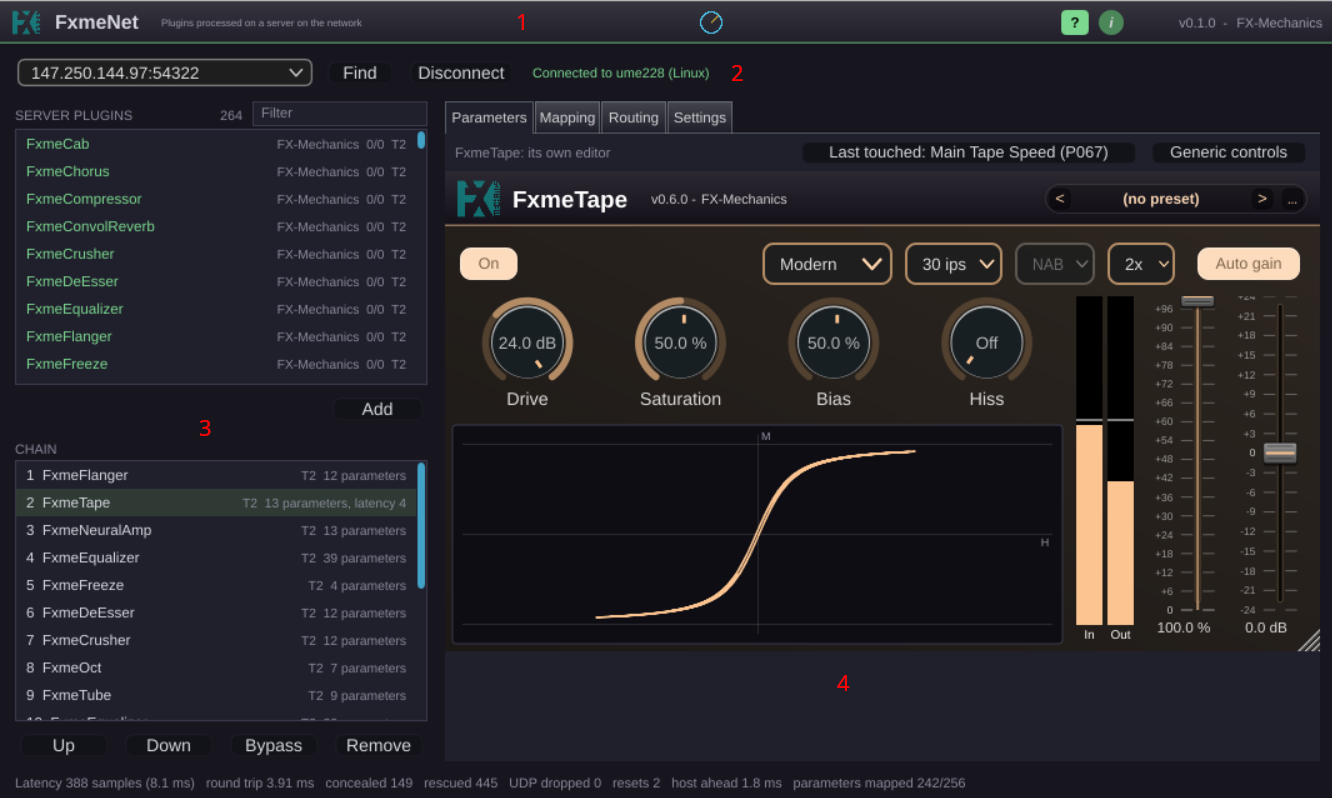
\includegraphics[width=\textwidth]{../img/fxme-net-plugin-screen.png}

From top to bottom:

\begin{description}
  \item[Top bar.] The FX-Mechanics logo and version, a \ui{?} switch that
    turns the hover help on or off for all instances, and an information
    button.
  \item[Server row.] The server's address, \ui{Find} and \ui{Connect} (the
    button reads \ui{Disconnect} while connected), and the connection
    status.
  \item[Left column.] \ui{SERVER PLUGINS}, the list of what the server offers,
    with its filter and the \ui{Add} button; and \ui{CHAIN}, your plugins
    in processing order, with \ui{Up}, \ui{Down}, \ui{Bypass} and
    \ui{Remove}.
  \item[Right side.] Four tabs: \ui{Parameters}, \ui{Mapping}, \ui{Routing}
    and \ui{Settings}.
  \item[Bottom line.] Statistics (section~\ref{sec:stats}).
\end{description}

\section{Connecting}

Type the server's address (a name or an IP address, with \cmd{:port} if it
does not use the default) or press \ui{Find} and choose a server from the
list that appears. \ui{Connect} opens the session. While the plugin is not
connected, the audio passes through untouched. The plugin remembers the last
server you used, on this computer, and connects again when you reopen a
project.

If the connection drops, the plugin reconnects by itself and resumes its
session when the server still has it (section~\ref{sec:sessions}).

\section{Choosing plugins}

\ui{SERVER PLUGINS} lists what the server offers. Each row shows the plugin's
name, its vendor, its input and output channels, and a tag \tier{2},
\tier{1} or \tier{0} that says how the plugin can be shown on this computer
(chapter~\ref{ch:tiers}). Hover over a row to see why it has its tier.

The list is sorted by tier (\tier{2} first, then \tier{1}, then \tier{0}) and
by name inside each tier. While the plugin scans this computer for the first
time, the order is by name only, and the tags read \tier{?}.

To find a plugin quickly, type a few letters in the \ui{Filter} field above
the list. Only plugins whose name contains every word you type remain. The
first match is selected: press \key{Return} to add it. \key{Esc} clears the
filter. \ui{Add} (or a double-click) adds the selected plugin at the end of
the chain.

\section{The chain}

\ui{CHAIN} lists your plugins in the order the server processes them, from
top to bottom. Select one to see its controls on the right. Buttons under
the list:

\begin{description}
  \item[Up, Down] Move the selected plugin in the chain.
  \item[Bypass] Bypass the selected plugin, on the server.
  \item[Remove] Remove it. The state of the plugin is lost.
\end{description}

A plugin that cannot be loaded on the server shows the reason in red (a
missing licence, a plugin that failed to start, ...).

The routing between the plugins is serial by default, as in a plain chain. To
do parallel processing or sidechains, see chapter~\ref{ch:routing}.

\section{The Parameters tab}

The tab shows the selected plugin.

\begin{itemize}
  \item If the plugin is installed on this computer in the same version
    (tier \tier{1} or \tier{2}), you see its own editor. It is a local copy,
    kept in step with the server: what you change in it is sent to the
    server, and what changes on the server appears in it. The window grows
    to fit the editor and returns to its normal size when you leave it.
  \item Otherwise, you see generic controls: one row per parameter with its
    name, a slider and its value. Double-click a slider to return to the
    default.
\end{itemize}

A button above the controls switches between the plugin's own editor and the
generic controls. A \ui{last touched} button next to it names the control you
moved last in the plugin's editor, with a menu to map it to an automation
parameter (below).

\section{Automation}

The DAW sees \fxme\ as one plugin with 256 automation parameters, named
\texttt{p001} to \texttt{p256} until they are used. When a plugin joins the
chain, its automatable parameters take the first free entries, and the DAW
shows them under the plugin's name (for example ``FxmeCompressor: Ratio'').
You can automate them, and the DAW's own controls, as with any plugin.

The \ui{Mapping} tab lists every entry in use and what it controls. To free
entries, select them and press \ui{Unmap}, or use \ui{Unmap all}.

To map a parameter by hand, use one of the two methods:

\begin{itemize}
  \item In the generic controls, press \ui{Map} on a row to give it the first
    free entry.
  \item Press \ui{Learn}, then move any of \fxme's parameters in the DAW: the
    parameter you moved becomes the one that controls it.
\end{itemize}

\begin{note}
Automation lanes in the DAW belong to the numbered entries. When you remove a
plugin, its entries stay free but keep their lane. \fxme\ does not give a
used entry to the next plugin you add (unless you map it by hand or all 256
have been used), so a recorded automation cannot silently drive another
plugin's parameter.
\end{note}

\section{Settings}

The \ui{Settings} tab has three parts.

\begin{description}
  \item[Stream.] \ui{Block size N} and \ui{Network budget D}, with the latency
    they give (chapter~\ref{ch:performance}).
  \item[Transport.] \ui{Silence in-flight audio at reset}: when the DAW restarts
    playback or jumps, drop the audio still on its way back from the server,
    so you hear silence for the length of the latency (as a local plugin
    clearing its delay line) rather than the tail of the previous position.
    \ui{Log transport events} writes what the audio thread sees around
    transport events, concealed blocks included, to
    \file{fxmenet-client-events.log} in the FX-Mechanics settings folder; it
    is for diagnosing problems.
  \item[Local plugins.] The scan of the plugins installed on \emph{this}
    computer, used for the plugins' own editors. \ui{Rescan} looks for new or
    changed plugins; \ui{Full rescan} examines everything again;
    \ui{Folders\ldots} adds folders to search beside the standard VST3 ones.
\end{description}

\section{Statistics}
\label{sec:stats}

The line at the bottom of the window gives:

\begin{description}
  \item[Latency] What \fxme\ reports to the DAW, in samples and milliseconds.
  \item[Round trip] The last measured time for a message to reach the server
    and come back.
  \item[Concealed] Blocks that came back too late and were replaced.
  \item[Rescued] Blocks that would have been concealed but arrived in time
    after a short wait.
  \item[UDP dropped] Audio messages the client threw away because they could not be put together: pieces missing, damaged or too large. It should stay at zero on a healthy network.
  \item[Resets] How many times the DAW reset the plugin (playback start, stop or a jump in the timeline). Each time, the server resets its chain at the same point of the stream.
  \item[Host ahead] How far the DAW processes audio ahead of real time, in milliseconds. It is 0 when the DAW calls the plugin at the pace of the sound card, and larger when the DAW renders with a read-ahead buffer.
  \item[Parameters mapped] How many of the 256 entries are in use.
\end{description}

A concealed count that rises steadily means the server or the network cannot
keep up with the chosen settings (chapter~\ref{ch:performance}).

\section{Bypass, projects and offline rendering}

\begin{itemize}
  \item \textbf{DAW bypass.} When you bypass \ui{FxmeNet} in the DAW, the
    plugin passes the audio dry, delayed by the same latency, so that
    switching it on and off does not move the track in time.
  \item \textbf{Saving.} The project stores the server, the settings, each
    plugin with its state, the parameter mapping and the routing. When you open
    the project, the plugin rebuilds the chain on the server and connects. If
    the server is not reachable then, the plugin keeps the state, and you can
    connect later.
  \item \textbf{Offline rendering.} When the DAW renders faster than real
    time (a bounce or an export), the plugin waits for each reply, so
    nothing is concealed and the result is exact.
\end{itemize}

\section{The same project on another computer}
\label{sec:sessions}

A project that uses \fxme\ needs the server to be reachable and to have the
same plugins installed. If a plugin is missing on the server, its row in the
chain shows an error and the audio is not processed by it. The audio goes through that position of the chain unchanged, as if the plugin were bypassed, and the rest of the chain keeps working. A future release will let you optionally compute the chain locally on the client when the server is not available.

\chapter{Routing}
\label{ch:routing}

By default the chain is serial, like the inserts of a mixer channel: the
output of each plugin feeds the next one, and the last one feeds the DAW.
The \ui{Routing} tab turns the chain into a patchbay, so that you can run
plugins in parallel, feed a sidechain from the DAW or from another plugin,
or send the outputs of a multi-output plugin to different channels.

\section{The view}

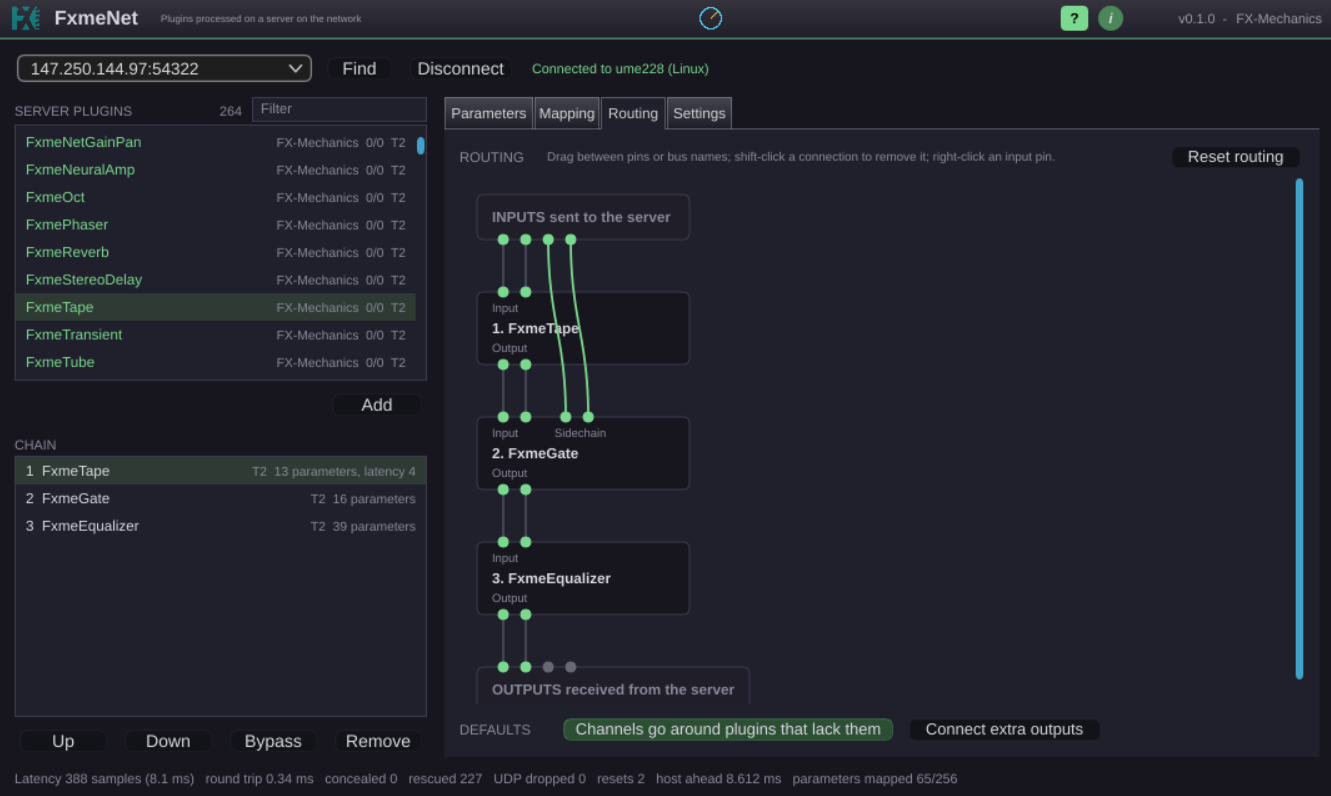
\includegraphics[width=\textwidth]{../img/fxme-net-routing-screen.png}

From top to bottom, the tab shows:

\begin{itemize}
  \item \textbf{Inputs}: the channels sent to the server (the plugin's input
    channels in the DAW);
  \item one box for each plugin of the chain, in chain order, with small
    \emph{pins} for its inputs on top and for its outputs below, grouped by
    \emph{bus} (``Main'', ``Sidechain'', and so on);
  \item \textbf{Outputs}: the channels received from the server (the plugin's
    output channels in the DAW).
\end{itemize}

A connection runs from an output pin to an input pin that is \emph{below}
it. Connections cannot go back up, so there is no feedback loop.

\section{Making and removing connections}

\begin{itemize}
  \item \textbf{Connect:} drag from an output pin to an input pin.
  \item \textbf{Connect a whole bus:} drag from a bus name to another bus
    name (or to a pin). The channels connect in order, so a stereo link
    takes one drag.
  \item \textbf{Remove:} click a connection while holding \key{Shift}.
  \item \textbf{Right-click an input pin} to disconnect it, or to put it back
    to the default rule (\ui{Back to the default routing}).
  \item \ui{Reset routing} puts the default routing back.
\end{itemize}

An output can feed several inputs (each gets a copy). Several outputs on one
input are summed, as in a DAW; this is how parallel paths are mixed back
together.

A bypassed plugin keeps its pins and passes each input channel to the output
channel with the same number.

\section{The default routing}

Until you change anything, each input of a plugin is fed by the nearest
plugin above it that has a matching output channel (the Inputs count as the
top box). This reproduces the behaviour of an ordinary serial chain:

\begin{itemize}
  \item a plugin with fewer channels than the stream lets the other channels
    pass around it to the next plugin that has them;
  \item a mono plugin with two outputs gives the plugin below its second
    output, not the DAW's second channel;
  \item sidechain and other auxiliary inputs start unconnected.
\end{itemize}

Two options under \ui{DEFAULTS} change the default rule. They never affect
connections you made by hand.

\begin{description}
  \item[Channels go around plugins that lack them] On by default. Off: each
    plugin is fed only by the one right above it, so channels that no plugin
    processes are silent.
  \item[Connect extra outputs] Off by default. On: the extra outputs of a
    plugin continue its main ones, so a plugin with two main and two extra
    outputs feeds four channels below it.
\end{description}

\section{Editing the chain after wiring}

You can add, remove and move plugins after you have wired the chain.
Connections you did not touch follow the default rule in the new chain. For
the ones you made by hand:

\begin{itemize}
  \item when a plugin is removed, what came out of it is replaced by what
    fed the same channel of its input, as if it were bypassed for good;
  \item when a plugin is moved, connections that no longer run downward are
    dropped;
  \item an input that loses all its sources through an edit goes back to the
    default, so the audio keeps flowing. An input you emptied yourself
    stays empty.
\end{itemize}

\section{Sidechains and auxiliary buses}

A sidechain input only becomes active when you connect something to it:
connect a DAW channel (an input) to the plugin's sidechain bus to compress a
bass with a kick, for example. The server then enables that bus, which
prepares that plugin again; expect a brief gap on that plugin only.
Unconnected auxiliary buses stay disabled, because many plugins behave
differently with an enabled bus that carries silence.

The channels the plugin sends to the server are the ones its connections
need. Channels you do not connect are not sent, which saves network
bandwidth.

\section{Latency and parallel paths}

When two paths of different latency meet at an input, \fxme\ delays the
shorter path so that they stay aligned. A parallel compressor, for example,
keeps its dry and wet signals in phase even when the processed path goes
through a linear-phase equaliser. The latency the DAW is told is the one of
the longest path from the inputs to the outputs.


\chapter{Latency, reliability and performance}
\label{ch:performance}

\fxme\ trades latency for reliability. This chapter explains the two
settings that control the trade, how to read what happens, and how to tune
the machines.

\section{Block size N and network budget D}

The plugin sends the audio to the server in blocks of N samples and gives
each reply D blocks of time to come back. Both are in the \ui{Settings}
tab.

\begin{description}
  \item[Block size N] 32 to 1024 samples. A small block means less latency
    but more packets per second and tighter deadlines for the server and
    the network.
  \item[Network budget D] 1 to 8 blocks. A larger budget survives a slower
    network or a busier server, at the price of more latency.
\end{description}

The latency that \fxme\ reports to the DAW is roughly N times D samples
plus the DAW's own block size, plus the latency of the chain's plugins. The
\ui{Settings} tab shows the exact figure for your settings, in samples and
milliseconds, split between the network and re-blocking part and the chain
itself. The DAW compensates for all of it, so the track stays in time; what
changes is how late a played instrument is heard, which matters when you
record through the plugin.

If a reply is not back in time, that block is \emph{concealed}: a short fade
to silence (64 samples) and back, so that there is no click, only a
very brief dip. Concealed blocks are counted on the bottom line of the
window.

The default is N\,=\,128 and D\,=\,2 (5.8\,ms of budget at 44.1\,kHz).

\section{Choosing the settings}

\begin{longtable}{@{}p{0.3\textwidth}p{0.64\textwidth}@{}}
\toprule
\textbf{Situation} & \textbf{Suggested settings}\\
\midrule
\endhead
Mixing, many heavy tracks & 1024$\times$2 or 512$\times$2: the most robust. Latency is no concern while mixing.\\
Recording through the plugin, light chain & 128$\times$2, or 64$\times$2 if the server has a lot of spare CPU.\\
A server near full load & Larger blocks. A busy server sometimes stalls for 20 to 50\,ms, which small blocks cannot absorb.\\
Network with other traffic or Wi-Fi & Raise D, or move to a wired connection.\\
\bottomrule
\end{longtable}

\begin{tip}
Test with the DAW's own settings in mind: the DAW's audio buffer adds to
\fxme's latency. Using a large buffer in the DAW for mixing and a small one
for recording is common practice, and works the same here.
\end{tip}

\section{Measured performance}

These figures come from the first stress tests (details in the project's
\file{doc/Tests} folder), on old machines: a 2015 Intel Core i7-6700K for the
client (Windows, Reaper, an RME ASIO interface at 44.1\,kHz and a buffer of
128) and a 2018 AMD Ryzen 5 PRO 2400G for the server (Ubuntu 24.04, four
cores). Every track had one \ui{FxmeNet} instance, and the ``full chain''
holds all 17 plugins of the FxmeFX collection (FX-Mechanics' effects).

\begin{longtable}{@{}p{0.22\textwidth}p{0.12\textwidth}p{0.14\textwidth}p{0.4\textwidth}@{}}
\toprule
\textbf{Tracks} & \textbf{Chain} & \textbf{N$\times$D} & \textbf{Result}\\
\midrule
\endhead
24 local & full & (local) & 75\,\% of the client's CPU.\\
24 remote & full & 256$\times$2 & Client at 25\,\%, server at about 66\,\%, about 10 concealed blocks in 5 minutes on one track.\\
24 remote & full & 1024$\times$2 & Client under 20\,\%, almost no concealed blocks.\\
28 remote & full & 1024$\times$2 & Server above 75\,\%: no concealed blocks, or very rare ones. Very usable.\\
32 remote & one equaliser & 128$\times$2 & Network at 95\,Mbit/s each way, no problem.\\
\bottomrule
\end{longtable}

What these tests show:

\begin{itemize}
  \item The offload works: the client's processor load fell from 75\,\% to
    20 to 25\,\% for the same session.
  \item Heavy loads (28 tracks with 17 plugins each, 476 plugin instances)
    are very usable with large blocks.
  \item Small blocks need headroom. While the server has spare CPU, 128 and
    256 work well; close to full load the server stalls for a few tens of
    milliseconds now and then, which short deadlines cannot absorb.
  \item These are extreme loads. Real sessions rarely put 17 plugins on every
    track.
\end{itemize}

\section{Making the server reliable (Linux)}
\label{sec:linuxtuning}

A generic Linux system works. These are the usual steps for audio on Linux;
try them one at a time and check after each whether the concealed count goes
down. More testing will be done. Feedback is welcome on the performance you get on other systems and with other optimizations.

\begin{enumerate}
  \item \textbf{Real-time priority for the audio threads.} Check with
\begin{lstlisting}
ps -eLo tid,cls,rtprio,pcpu,comm | grep -i fxme
\end{lstlisting}
    while a session is open: the audio threads should be in class \cmd{RR}
    or \cmd{FF}. If they are \cmd{TS}, the system refused real-time priority
    (the server's log says so). Create
    \file{/etc/security/limits.d/audio.conf}:
\begin{lstlisting}[language={}]
@audio - rtprio 95
@audio - memlock unlimited
\end{lstlisting}
    Add the account that runs the server to the \cmd{audio} group, and log in
    again (or restart the service).
  \item \textbf{Bigger socket buffers.} Under heavy load the kernel can drop
    replies when the send buffer is full (the server's log counts them as
    \emph{send errors}; \cmd{nstat -az UdpSndbufErrors} shows the
    system-wide count). Raise the limits, then restart the server:
\begin{lstlisting}
sudo sysctl -w net.core.rmem_default=4194304 net.core.rmem_max=8388608
sudo sysctl -w net.core.wmem_default=4194304 net.core.wmem_max=8388608
\end{lstlisting}
    To keep them after a reboot, put the four lines (without \cmd{sudo
    sysctl -w}) in \file{/etc/sysctl.d/90-fxmenet.conf}.
  \item \textbf{CPU frequency.} Set the governor to performance:
\begin{lstlisting}
sudo cpupower frequency-set -g performance
\end{lstlisting}
  \item \textbf{Kernel.} A low-latency or fully preemptible kernel
    (\cmd{linux-lowlatency}, or booting with \cmd{preempt=full}) helps the
    worst cases.
\end{enumerate}

\todo{When the server asks for large socket buffers itself (todo item 21),
step 2 becomes: ``the log tells you if the system limits are too low''.}

\section{Making the client reliable}

\begin{itemize}
  \item Use a wired gigabit connection, and keep other heavy traffic off it.
  \item In Reaper, try turning off \emph{anticipative FX processing} for the
    tracks that hold \ui{FxmeNet}, and compare the concealed counts.
  \item On the network adapter, turn interrupt moderation off or to low, and
    use the high-performance power plan.
\end{itemize}

\chapter{Tiers: editors and meters}
\label{ch:tiers}

Every plugin in the server's list carries a tag, \tier{0}, \tier{1} or
\tier{2}. It says what you can have on the client for that plugin.

\begin{longtable}{@{}p{0.08\textwidth}p{0.88\textwidth}@{}}
\toprule
\textbf{Tier} & \textbf{What you get}\\
\midrule
\endhead
\tier{2} & The plugin's own editor on the client, with its meters, spectra and other displays showing the server's real signal. The plugin is made for \fxme\ (chapter~\ref{ch:developers}) and installed in the same version on the client.\\
\tier{1} & The plugin's own editor on the client, kept in step with the server's copy. Meters and analysers that read the audio inside the plugin stay empty, since the audio is not on the client.\\
\tier{0} & Generic controls: a slider per parameter. Used when the plugin is not installed on the client, or is another version.\\
\bottomrule
\end{longtable}

\section{How the plugin decides}

The plugin scans the VST3 folders of the computer that runs the DAW. A server
plugin matches a local one when the identifier, the name and the vendor are
the same. The version then decides:

\begin{itemize}
  \item the same version, and the server says the plugin is made for \fxme:
    tier \tier{2};
  \item the same version otherwise: tier \tier{1};
  \item another version, or no local copy: tier \tier{0}.
\end{itemize}

When both computers run the same operating system, the plugin also compares
the binary files. A difference (another build of the same version) is shown
on hover but does not stop the plugin from being used. Hover over a row of
the list to see the reason for its tier.

The \ui{FxmeNet} plugin itself is never listed, and neither are instruments.

\section{What the local copy does}

For tiers \tier{1} and \tier{2}, the plugin creates a local copy of the
server's plugin when you first open its editor. This \emph{mirror} never
processes audio; it only shows the editor. Your changes go to the server,
and the server's state comes back to the mirror. For a plugin made for
\fxme, whatever the plugin changes outside its parameters (a preset, a loaded
file) is copied to the server in full.

\begin{note}
Install the same plugin versions on both machines. A tier \tier{1} or
\tier{2} editor on a different version is a source of surprises, so \fxme\
does not use it; the plugin shows as tier \tier{0}.
\end{note}

\section{Keeping the plugin list up to date}

If you install a plugin on the client while the DAW runs, use \ui{Rescan} in
the \ui{Settings} tab, and the tags update. If your plugins live in a
folder that is not standard, add it with \ui{Folders\ldots}.

\chapter{For plugin developers}
\label{ch:developers}

\fxme\ runs any VST3 effect. A plugin can also be made \emph{\fxme-aware}, and
then it gets tier \tier{2} (chapter~\ref{ch:tiers}): its editor on the
client shows the live meters, spectra and values of the copy that runs on
the server. This chapter summarises what that takes. The reference is the
file \file{fxmenet-howto.md} of FxmeTools, with the demonstration plugin
\file{Examples/GainPan} in the \fxme\ source.

\section{The idea}

The plugin is loaded twice: a \emph{source} on the server, which processes
audio, and a \emph{mirror} on the client, which never processes and shows
the editor. What the editor reads that is not a parameter (a meter, a
spectrum, a computed value) is sent from the source to the mirror as
telemetry and written into the mirror's own objects, so the editor itself
does not change. Outside \fxme\ the plugin behaves exactly as before.

\section{What to do}

\begin{enumerate}
  \item Add an \texttt{fxme::net::NetBridge} to the processor, and return it from
    \texttt{getVST3Client\allowbreak Extensions()}.
  \item Register everything the editor reads that is not a parameter, with a
    stable name each: meters, taps, atomics, computed scalars.
  \item In the few getters that compute from the DSP, return the telemetry
    value when the plugin is a mirror.
  \item Skip the work that only feeds the DSP when the plugin is a mirror.
  \item Call \texttt{notifyStateChanged()} when state that is not a parameter
    changes (a loaded file, for example).
\end{enumerate}

\begin{lstlisting}[style=fxcode]
#include <FxmeTools/net/NetBridge.h>

class MyProcessor : public juce::AudioProcessor
{
public:
    juce::VST3ClientExtensions* getVST3ClientExtensions() override { return &net; }
private:
    Compressor compressor;
    fxme::net::NetBridge net;   // after everything it registers
};

MyProcessor::MyProcessor()
{
    net.telemetry().addMeter ("gr", compressor.getGrMeter());
}
\end{lstlisting}

\begin{longtable}{@{}p{0.34\textwidth}p{0.6\textwidth}@{}}
\toprule
\textbf{The editor reads} & \textbf{Register}\\
\midrule
\endhead
a level meter & \texttt{addMeter (name, meter)}\\
a spectrum or waveform tap & \texttt{addTap (name, tap)}\\
a \texttt{std::atomic<float>} & \texttt{addValue (name, atomic)}\\
a function that computes a value & \texttt{addScalar (name, getter)}\\
a read-and-reset function & \texttt{addPeak (name, function)}\\
\bottomrule
\end{longtable}

\section{Checking}

The \fxme\ source includes a test tool, \cmd{FxmeNetLoopback}, which loads
your plugin twice in one process, as source and mirror, and pumps the
telemetry between them. Both editors appear side by side; the mirror's
meters must follow the source's.

\begin{lstlisting}
FxmeNetLoopback path/to/MyPlugin.vst3
\end{lstlisting}

\section{The \fxme\ compatible mark}
\label{sec:stamp}

Plugins that support \fxme\ may carry the \fxme\ mark, so that users know the
plugin gives a tier \tier{2} experience.

\begin{center}
  \fxlogo[width=0.28\textwidth]{FxmeNetLogo3.jpg}\qquad
  \fxlogo[width=0.08\textwidth]{fxmenet-logo.png}
\end{center}

\todo{The two marks above are drafts (a connector-shaped logo and a small
icon). Decide the final design and supply it as SVG and as transparent PNG in
several sizes. Write the conditions of use: what a plugin must do to carry it
(for example, that it passes the Loopback check and that its editor works
as a mirror), where to show it (website, manual, plugin's information
panel), and the licence of the artwork.}

\chapter{Troubleshooting}
\label{ch:troubleshooting}

\section{The plugin does not find the server}

\begin{itemize}
  \item Is the server running? On its machine, \cmd{fxmenet-top} should show
    it. If not, start \cmd{fxmenet-server}.
  \item Does \ui{Find} show nothing? Discovery uses a broadcast, which does not
    cross routers or most VPNs, and is blocked by some firewalls. Type the
    server's address in the field instead.
  \item Can the client reach the server's ports? Check the firewall on the
    server (TCP 54322, UDP 54321 and 54320) and, on the client, that the
    DAW is allowed to use the network.
  \item Is a second server running on the same machine? Only one can answer
    \ui{Find}; give the other one a different port set, or no discovery.
\end{itemize}

\section{The plugin I want is not in the list}

\begin{itemize}
  \item It must be a VST3 \emph{effect} installed on the server, in a folder
    the server searches (section~\ref{sec:folders}).
  \item Look at the server's log (or the \key{3} view of
    \cmd{fxmenet-top}) for ``skipped'': a plugin that crashed or hung when
    loaded is left out until it changes.
  \item You installed it while the server ran: rescan with \key{r} in
    \cmd{fxmenet-top}, then reconnect the plugin.
  \item The list is filtered: clear the \ui{Filter} field.
\end{itemize}

\section{A plugin shows tier \tier{0} when I expected \tier{1}}

The plugin must be installed on the client, in a folder the client scans, in
the same version. Hover over the row for the reason. Use \ui{Rescan} or
\ui{Folders\ldots} in the \ui{Settings} tab (chapter~\ref{ch:tiers}).

\section{Concealed blocks, dropouts or clicks}

Look at where the problem is.

\begin{enumerate}
  \item In \cmd{fxmenet-top}, is the server's CPU high, or a session's load bar
    red? Then the server is overloaded: use larger blocks (1024$\times$2),
    reduce the load, or use a faster server.
  \item Does a session's \emph{lost} count rise? Requests do not reach the
    server in time: look at the network (wired? other traffic? a switch
    that drops packets?).
  \item Does \emph{send errors} rise in the server's log? The kernel drops
    replies: raise the socket buffers (section~\ref{sec:linuxtuning}).
  \item Do the threads show \cmd{TS} instead of \cmd{RR} in the check of
    section~\ref{sec:linuxtuning}? Give the audio threads real-time priority.
  \item Only the client's concealed count rises while the server's counts are
    zero? Replies are delayed on their way back, or the server stalls
    briefly. Raise D by one.
\end{enumerate}

If clicks persist, enable \ui{Log transport events} in the \ui{Settings}
tab, reproduce the problem, and keep \file{fxmenet-client-events.log} and the
server's log together for the report.

\section{Silence at start, stop or jump}

This is the \ui{Silence in-flight audio at reset} option of the
\ui{Settings} tab doing its job: for the length of the latency after a
restart, nothing is heard from the plugin, as with a local plugin whose delay
line is cleared. Turn the option off to hear what was still in flight.

\section{The audio is late compared with other tracks}

The DAW compensates for the latency that \fxme\ reports. If a track is
still late, check that the DAW's plugin delay compensation is on and that
the DAW applies it to this track.

\section{Everything stops when the server restarts}

The plugin reconnects by itself and rebuilds the chain on the server. If the
server does not have the same plugins any more, the affected plugins show an
error in the chain. While the server is away, the sound becomes dry at once; when the server is back, the processed sound returns. Restarting the server during playback was tested, without audible glitches.


\chapter{Reference}
\label{ch:reference}

\section{Files}

\begin{longtable}{@{}p{0.42\textwidth}p{0.52\textwidth}@{}}
\toprule
\textbf{File} & \textbf{Content}\\
\midrule
\endhead
\file{FX-Mechanics/fxmenet-server-plugins.xml} & The server's plugin cache.\\
\file{FX-Mechanics/fxmenet-server-settings.json} & The folders and the default-folders switch set with \cmd{fxmenet-top}.\\
\file{FX-Mechanics/FxmeNet.settings} & Client: the last server, the hover-help switch, the extra plugin folders (machine-wide).\\
\file{FX-Mechanics/fxmenet-client-plugins.xml} & Client: the cache of the local plugin scan.\\
\file{FX-Mechanics/fxmenet-client-events.log} & Client: the transport events log, when enabled.\\
\bottomrule
\end{longtable}

\noindent The \file{FX-Mechanics} folder is in the user's application-data
folder (on Linux, \file{~/.config}; on Windows,
\file{%APPDATA%}; on macOS, \file{~/Library/Application Support}). \todo{verify these locations on each system}

\section{Ports}

See chapter~\ref{ch:network}.

\section{Limits}

\begin{itemize}
  \item 256 automation parameters per \ui{FxmeNet} instance.
  \item 1 to 64 channels in and out of each \ui{FxmeNet} instance (stereo by
    default).
  \item Block sizes from 32 to 1024 samples; a network budget of 1 to 8 blocks.
  \item Plugins: VST3 effects on the server.
\end{itemize}

\section{More documentation}

The project's \file{doc} folder holds the technical documents:
\file{architecture.md} (how the code is built), \file{protocol.md} (the wire
protocol, for anyone writing another client or tool), \file{routing.md} (the
design of the routing) and \file{Tests/stress-tests.md} (the measurements of
chapter~\ref{ch:performance} in full).

\chapter{Network requirements}
\label{ch:network}

\section{Ports}

\begin{longtable}{@{}p{0.12\textwidth}p{0.14\textwidth}p{0.62\textwidth}@{}}
\toprule
\textbf{Port} & \textbf{Protocol} & \textbf{Use}\\
\midrule
\endhead
54320 & UDP & Discovery: answers the plugin's \ui{Find}. Optional.\\
54321 & UDP & Audio: requests and replies of all sessions, and telemetry.\\
54322 & TCP & Control: the plugin lists, parameters, state, and \cmd{fxmenet-top}.\\
\bottomrule
\end{longtable}

All three can be changed with the server's options (chapter~\ref{ch:server}).
The client opens connections to the server; the server only needs these three
ports open to the client.

\section{Bandwidth}

Audio travels as 32-bit floating-point samples, uncompressed, in both
directions: about 2.8\,Mbit/s for a stereo track at 44.1\,kHz, 3.1\,Mbit/s at
48\,kHz, and the more for more channels. In the first stress tests, 24
stereo tracks used about 71\,Mbit/s each way and 32 tracks used 95\,Mbit/s
each way. A gigabit connection carries several hundred tracks of this kind
in theory; in practice, the server's CPU and the quality of the network
limit the number of tracks first.

Only the channels that the routing uses are sent
(chapter~\ref{ch:routing}).

\section{Security}

The traffic is not encrypted or authenticated. A token in each session keeps
stray packets out, but anyone on the network can talk to the server. Use
\fxme\ on a network you trust, and keep the ports closed on the internet.

\chapter{Glossary}
\label{ch:glossary}

\begin{description}
  \item[Aux bus] A plugin input or output beyond its main ones, such as a
    sidechain.
  \item[Block] A group of N samples sent to the server and returned.
  \item[Budget (D)] The number of blocks of time a reply has to come back.
  \item[Chain] The plugins of a session, in processing order.
  \item[Client] The \ui{FxmeNet} plugin in the DAW.
  \item[Concealed block] A block whose reply was late, replaced by a short
    fade to silence and back.
  \item[Control channel] The TCP connection that carries plugin lists,
    parameters and state.
  \item[Discovery] The broadcast that lets \ui{Find} locate servers.
  \item[Mirror] The local copy of a server plugin that shows its editor and
    never processes audio.
  \item[Monitor] A connection that watches a server without a session
    (\cmd{fxmenet-top}).
  \item[Pin] The place where a connection joins a plugin's input or output
    in the routing view.
  \item[Pool] The 256 automation parameters of an \ui{FxmeNet} instance.
  \item[Server] \cmd{fxmenet-server}.
  \item[Session] One \ui{FxmeNet} instance connected to the server.
  \item[Telemetry] The values (meters, spectra) a plugin made for \fxme\ sends
    from the server to its editor on the client.
  \item[Tier] \tier{0}, \tier{1} or \tier{2}: how a plugin can be shown on the
    client (chapter~\ref{ch:tiers}).
\end{description}


\end{document}
